\documentclass[10pt]{beamer}\usepackage[]{graphicx}\usepackage[]{color}
%% maxwidth is the original width if it is less than linewidth
%% otherwise use linewidth (to make sure the graphics do not exceed the margin)
\makeatletter
\def\maxwidth{ %
  \ifdim\Gin@nat@width>\linewidth
    \linewidth
  \else
    \Gin@nat@width
  \fi
}
\makeatother

\definecolor{fgcolor}{rgb}{0.345, 0.345, 0.345}
\newcommand{\hlnum}[1]{\textcolor[rgb]{0.686,0.059,0.569}{#1}}%
\newcommand{\hlstr}[1]{\textcolor[rgb]{0.192,0.494,0.8}{#1}}%
\newcommand{\hlcom}[1]{\textcolor[rgb]{0.678,0.584,0.686}{\textit{#1}}}%
\newcommand{\hlopt}[1]{\textcolor[rgb]{0,0,0}{#1}}%
\newcommand{\hlstd}[1]{\textcolor[rgb]{0.345,0.345,0.345}{#1}}%
\newcommand{\hlkwa}[1]{\textcolor[rgb]{0.161,0.373,0.58}{\textbf{#1}}}%
\newcommand{\hlkwb}[1]{\textcolor[rgb]{0.69,0.353,0.396}{#1}}%
\newcommand{\hlkwc}[1]{\textcolor[rgb]{0.333,0.667,0.333}{#1}}%
\newcommand{\hlkwd}[1]{\textcolor[rgb]{0.737,0.353,0.396}{\textbf{#1}}}%
\let\hlipl\hlkwb

\usepackage{framed}
\makeatletter
\newenvironment{kframe}{%
 \def\at@end@of@kframe{}%
 \ifinner\ifhmode%
  \def\at@end@of@kframe{\end{minipage}}%
  \begin{minipage}{\columnwidth}%
 \fi\fi%
 \def\FrameCommand##1{\hskip\@totalleftmargin \hskip-\fboxsep
 \colorbox{shadecolor}{##1}\hskip-\fboxsep
     % There is no \\@totalrightmargin, so:
     \hskip-\linewidth \hskip-\@totalleftmargin \hskip\columnwidth}%
 \MakeFramed {\advance\hsize-\width
   \@totalleftmargin\z@ \linewidth\hsize
   \@setminipage}}%
 {\par\unskip\endMakeFramed%
 \at@end@of@kframe}
\makeatother

\definecolor{shadecolor}{rgb}{.97, .97, .97}
\definecolor{messagecolor}{rgb}{0, 0, 0}
\definecolor{warningcolor}{rgb}{1, 0, 1}
\definecolor{errorcolor}{rgb}{1, 0, 0}
\newenvironment{knitrout}{}{} % an empty environment to be redefined in TeX

\usepackage{alltt}%
\setbeamersize{text margin left=0.5cm, text margin right=0.5cm}

\usepackage{alltt}%
\usetheme[background=light]{metropolis} 
\usecolortheme{seahorse}

\usepackage[utf8]{inputenc}%


\usepackage[normalem]{ulem}%strikeout
 

% graphics
%% Figures %%%%%%%%%%%%%%%%%%%%%%%%%%%%%%%%%%%%%%%%%%%%%%%%%%
\usepackage{graphicx}
\usepackage{xcolor}%for color mixing

\usepackage{amsmath}%
\usepackage{amsfonts}%
\usepackage{amssymb}%
\usepackage{graphicx}

\usepackage{tikz}
\usetikzlibrary{calc}

\usepackage{hyperref}

%%%%%%%%%%%%%%%%%%%%%%%%%%%%%%%%%%%%%%%%%%%%%%
%%%%%%%%%%%%%%%%% Doc info %%%%%%%%%%%%%%%%%%%
\title{Introduction to model selection in R}
\author{Timoth\'ee Bonnet}
\institute{BDSI / RSB}
\date{\today}

%%%%%%%%%%%%%%%%%%%%%%%%%%%%%%%%%%%%
\IfFileExists{upquote.sty}{\usepackage{upquote}}{}
\begin{document}



\begin{frame}
  \begin{quote}
  ``If a particular model (parametrization) does not make biological sense,
this is reason to exclude it from the set of candidate models, particularly
in the case where causation is of interest. In developing the set of candidate
models, one must recognize a certain balance between keeping the set small
and focused on plausible hypotheses, while making it big enough to guard
against omitting a very good a priori model."
  \end{quote}

Burnham and Anderson, 2002, Model Selection and Multimodel Inference: A Practical Information-theoretic Approach

\end{frame}
%%%%%%%%%%%

\begin{frame}
\maketitle
\end{frame}
%%%%%%%%%%%


\AtBeginSection[]
{
  \begin{frame}<beamer>
    \Large
    \frametitle{}
    \tableofcontents[currentsection,hideothersubsections,subsectionstyle=hide]% down vote\tableofcontents[currentsection,currentsubsection,hideothersubsections,sectionstyle=show/hide,subsectionstyle=show/shaded/hide]
  \end{frame}
}



%%%%%%%%%%%%%%%%%%%%%%%%%%%%%%%%%%%%%%%%%%%%%%%%%%%%%%%%%%%%%%%%%%%
%%%%%%%%%%%%%%%%%%%%%%%%%%%%%%%%%%%%%%%%%%%%%%%%%%%%%%%%%%%%%%%%%%%
\section{Why model selection?}

\begin{frame}{}




\end{frame}
%%%%%%%%%%%

\begin{frame}[fragile]{Overfitting}



\only<1>{
\begin{knitrout}\small
\definecolor{shadecolor}{rgb}{0.843, 0.867, 0.922}\color{fgcolor}
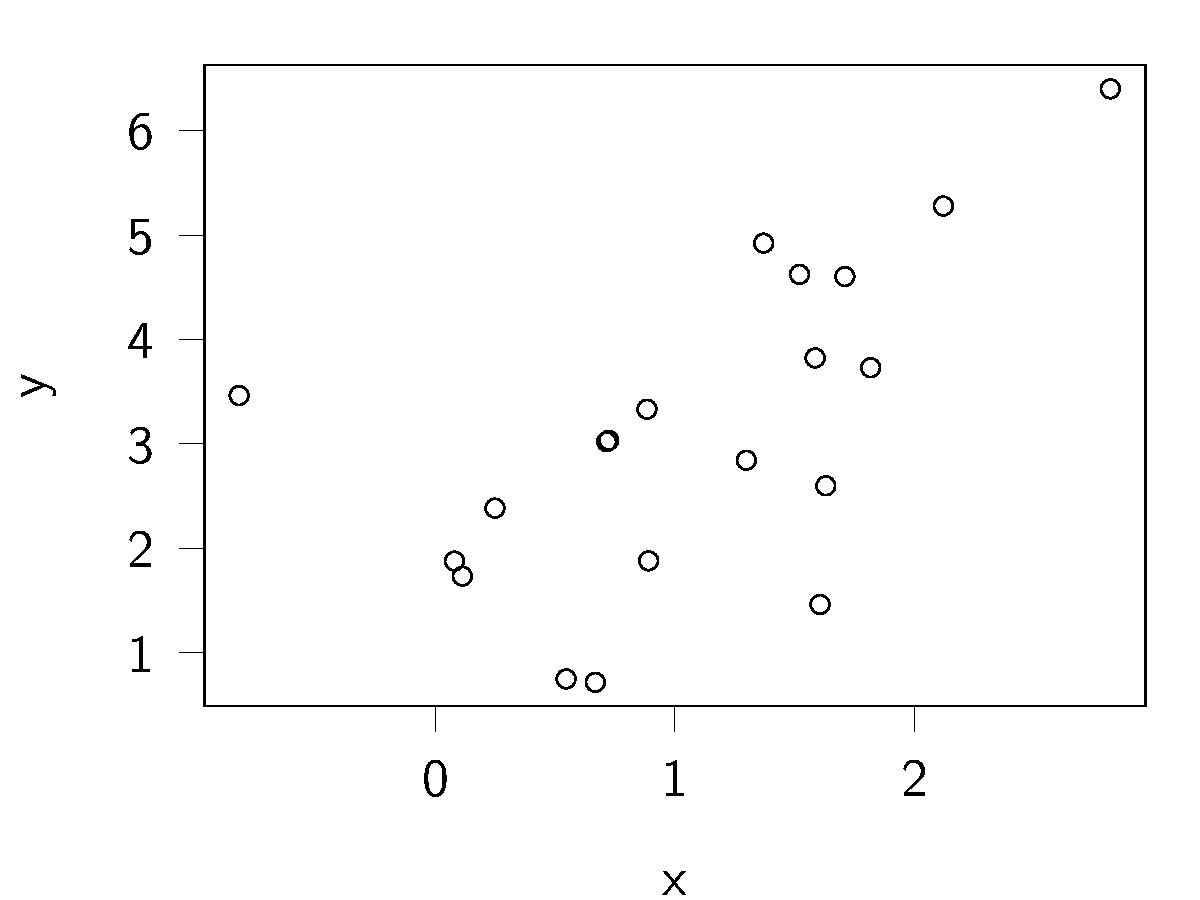
\includegraphics[width=0.8\textwidth,height=0.6\textwidth]{figure/model1-1} 

\end{knitrout}
}

\only<2>{
\begin{knitrout}\small
\definecolor{shadecolor}{rgb}{0.843, 0.867, 0.922}\color{fgcolor}
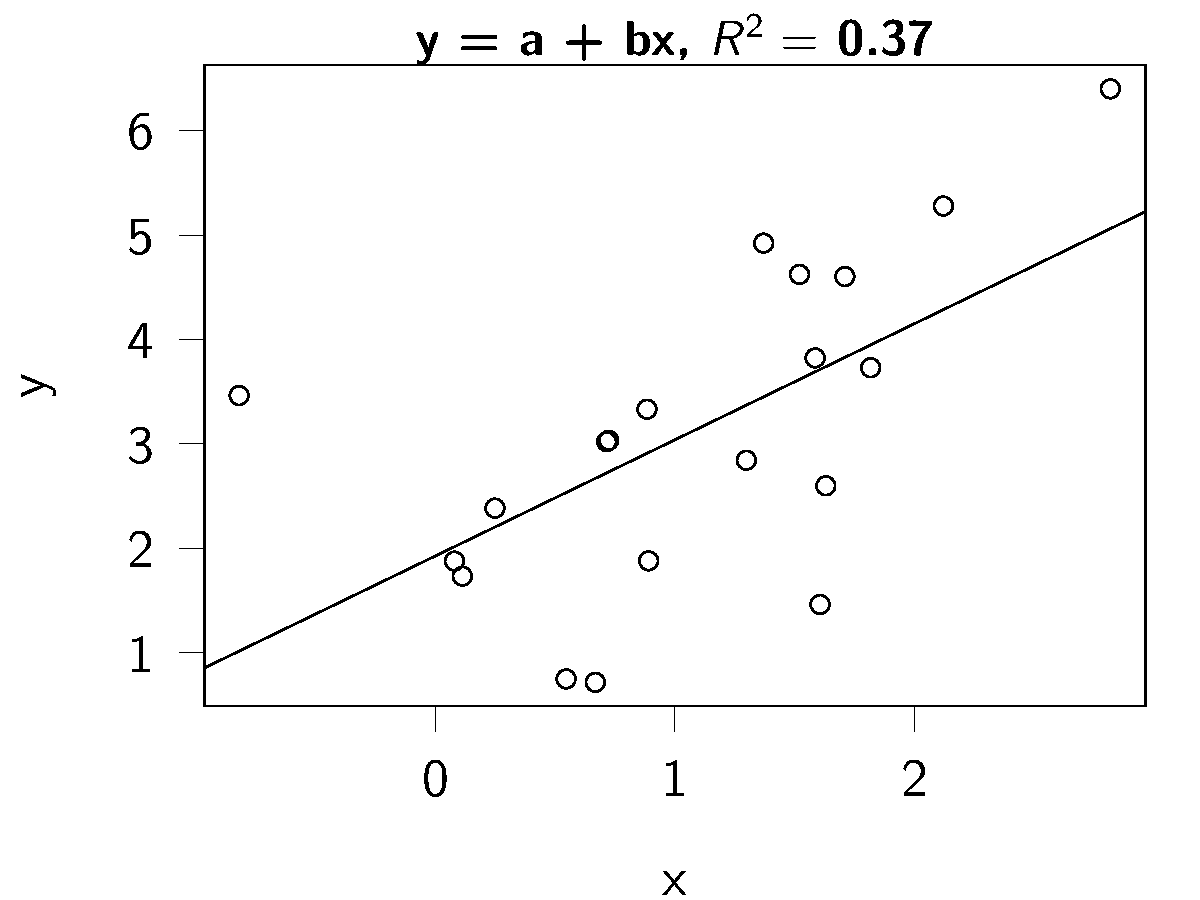
\includegraphics[width=0.8\textwidth,height=0.6\textwidth]{figure/model2-1} 

\end{knitrout}
}

\only<3>{
\begin{knitrout}\small
\definecolor{shadecolor}{rgb}{0.843, 0.867, 0.922}\color{fgcolor}
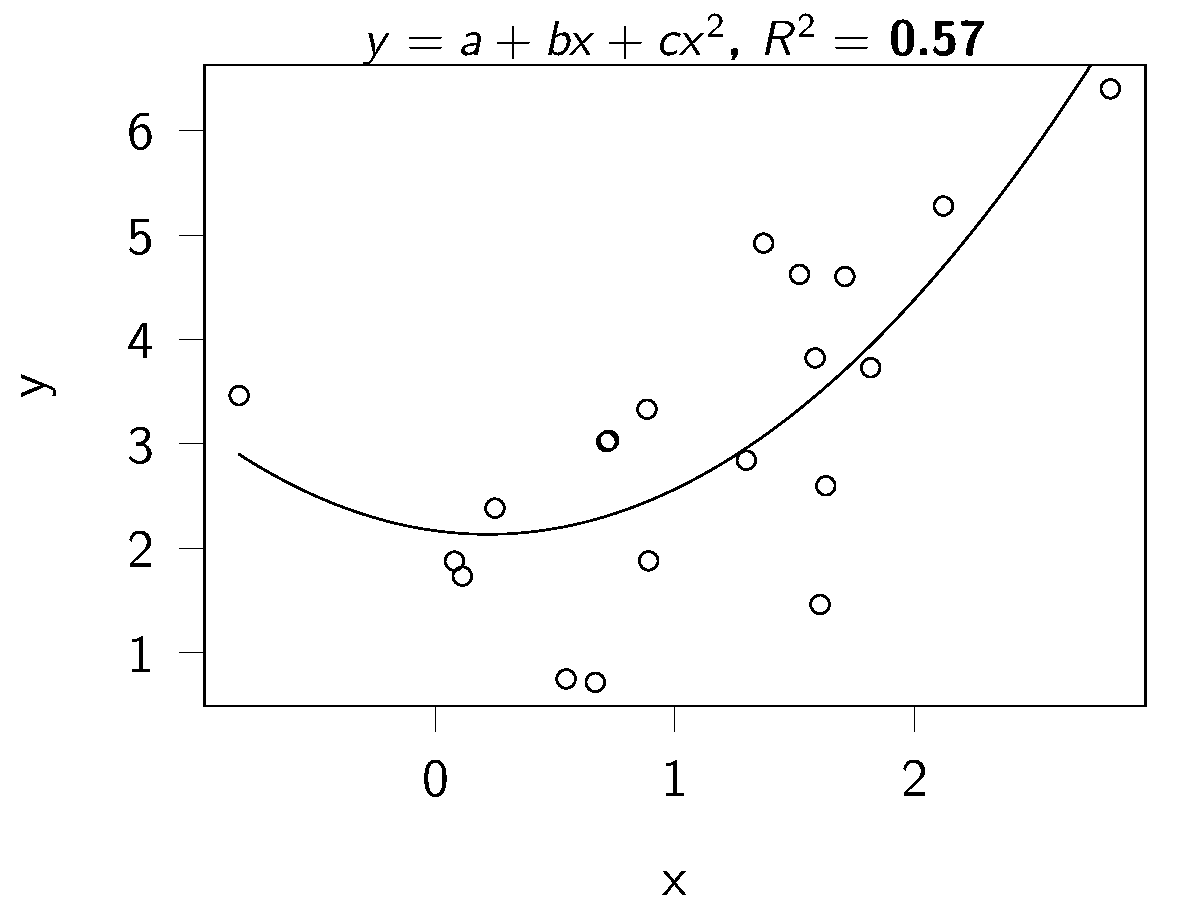
\includegraphics[width=0.8\textwidth,height=0.6\textwidth]{figure/model3-1} 

\end{knitrout}
}

\only<4>{
\begin{knitrout}\small
\definecolor{shadecolor}{rgb}{0.843, 0.867, 0.922}\color{fgcolor}
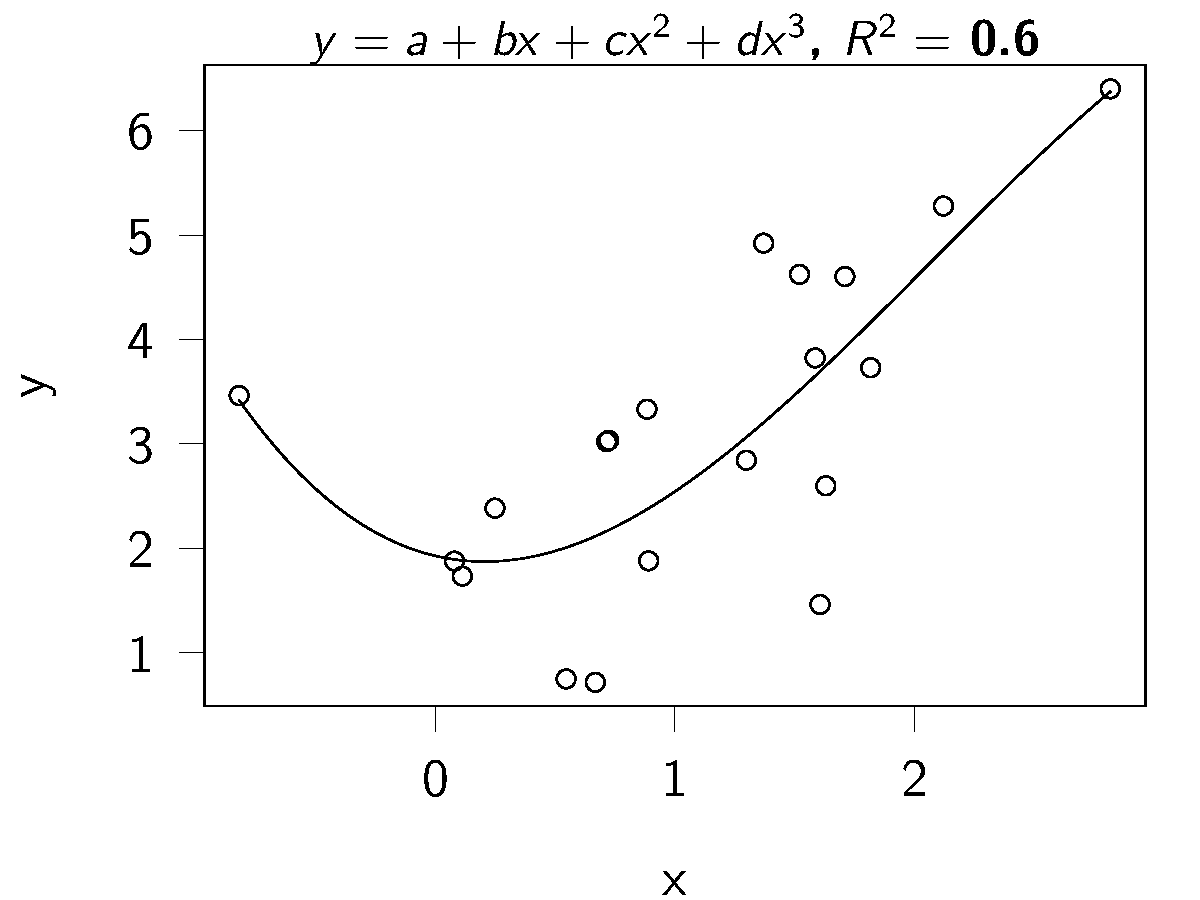
\includegraphics[width=0.8\textwidth,height=0.6\textwidth]{figure/model4-1} 

\end{knitrout}
}


\only<5>{
\begin{knitrout}\small
\definecolor{shadecolor}{rgb}{0.843, 0.867, 0.922}\color{fgcolor}
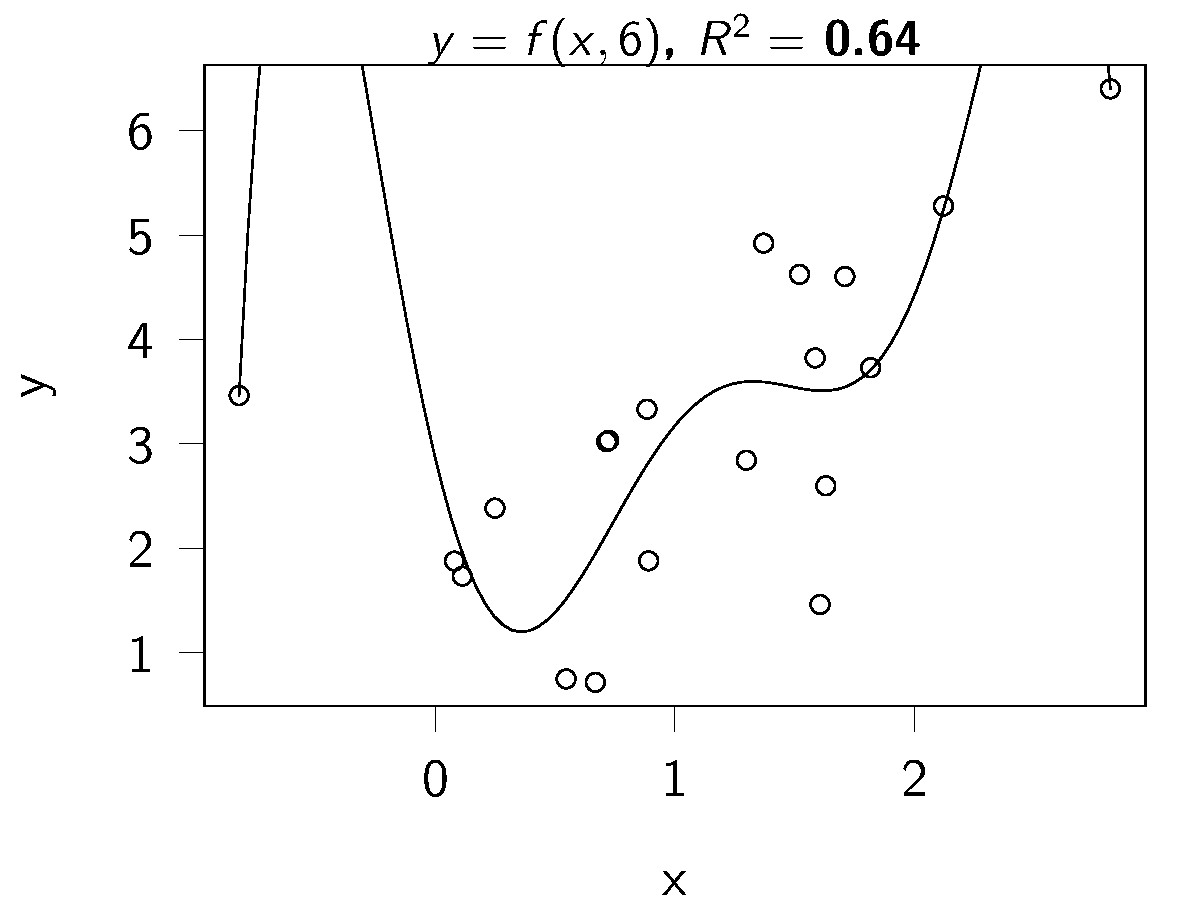
\includegraphics[width=0.8\textwidth,height=0.6\textwidth]{figure/model5-1} 

\end{knitrout}
}


\only<6>{
\begin{knitrout}\small
\definecolor{shadecolor}{rgb}{0.843, 0.867, 0.922}\color{fgcolor}
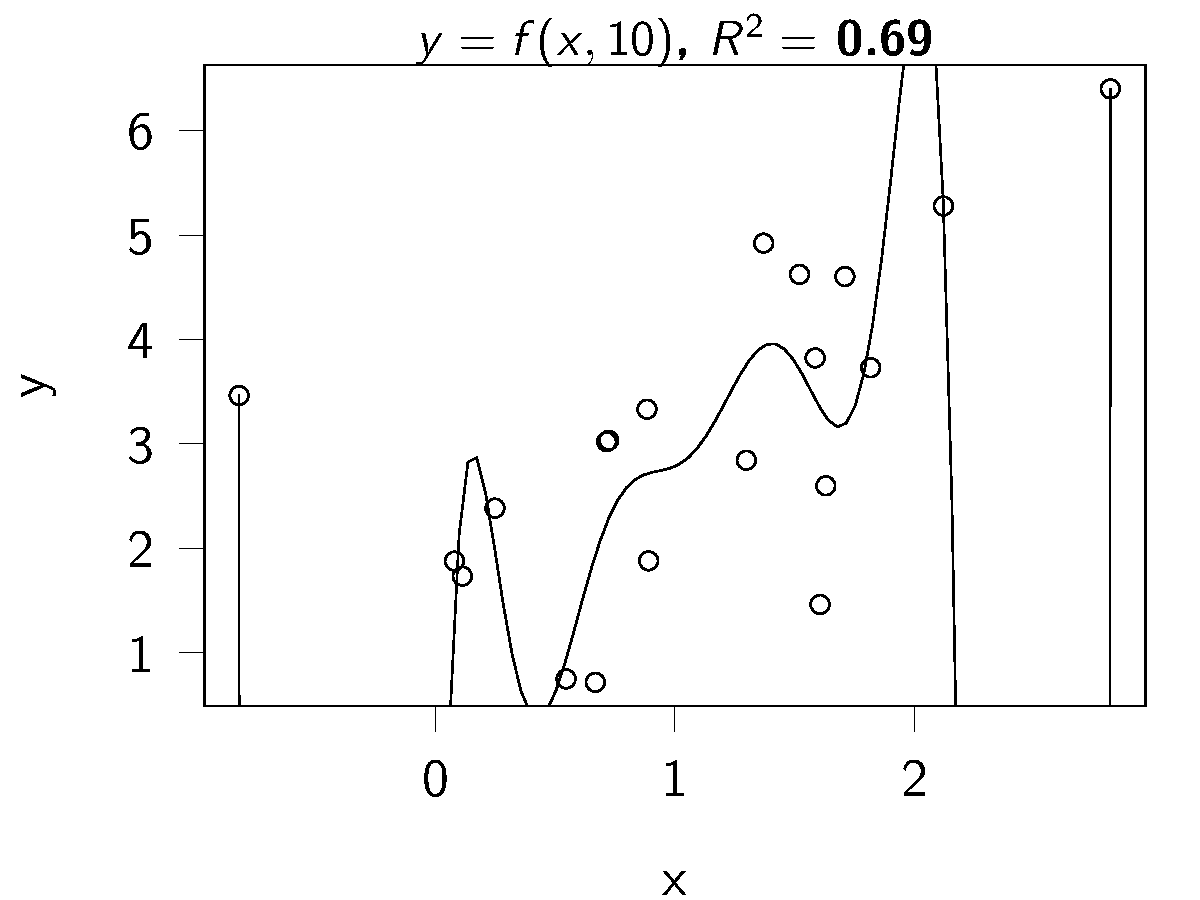
\includegraphics[width=0.8\textwidth,height=0.6\textwidth]{figure/model6-1} 

\end{knitrout}
}

\only<7>{
\begin{knitrout}\small
\definecolor{shadecolor}{rgb}{0.843, 0.867, 0.922}\color{fgcolor}
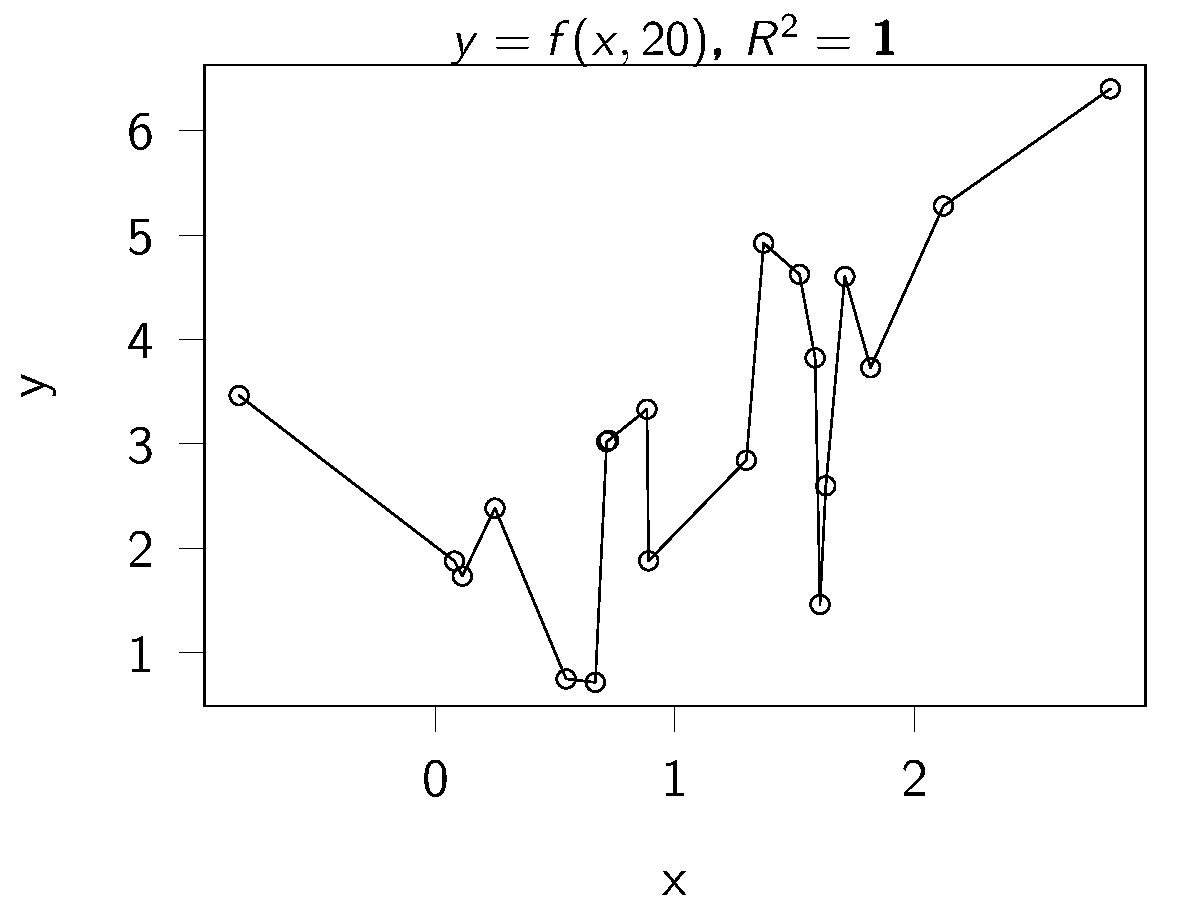
\includegraphics[width=0.8\textwidth,height=0.6\textwidth]{figure/model7-1} 

\end{knitrout}
}
\end{frame}
%%%%%%%%%%%%%

\begin{frame}[fragile]{Overfitting: What is wrong? Part 1}

\only<1>{
\begin{knitrout}\small
\definecolor{shadecolor}{rgb}{0.843, 0.867, 0.922}\color{fgcolor}
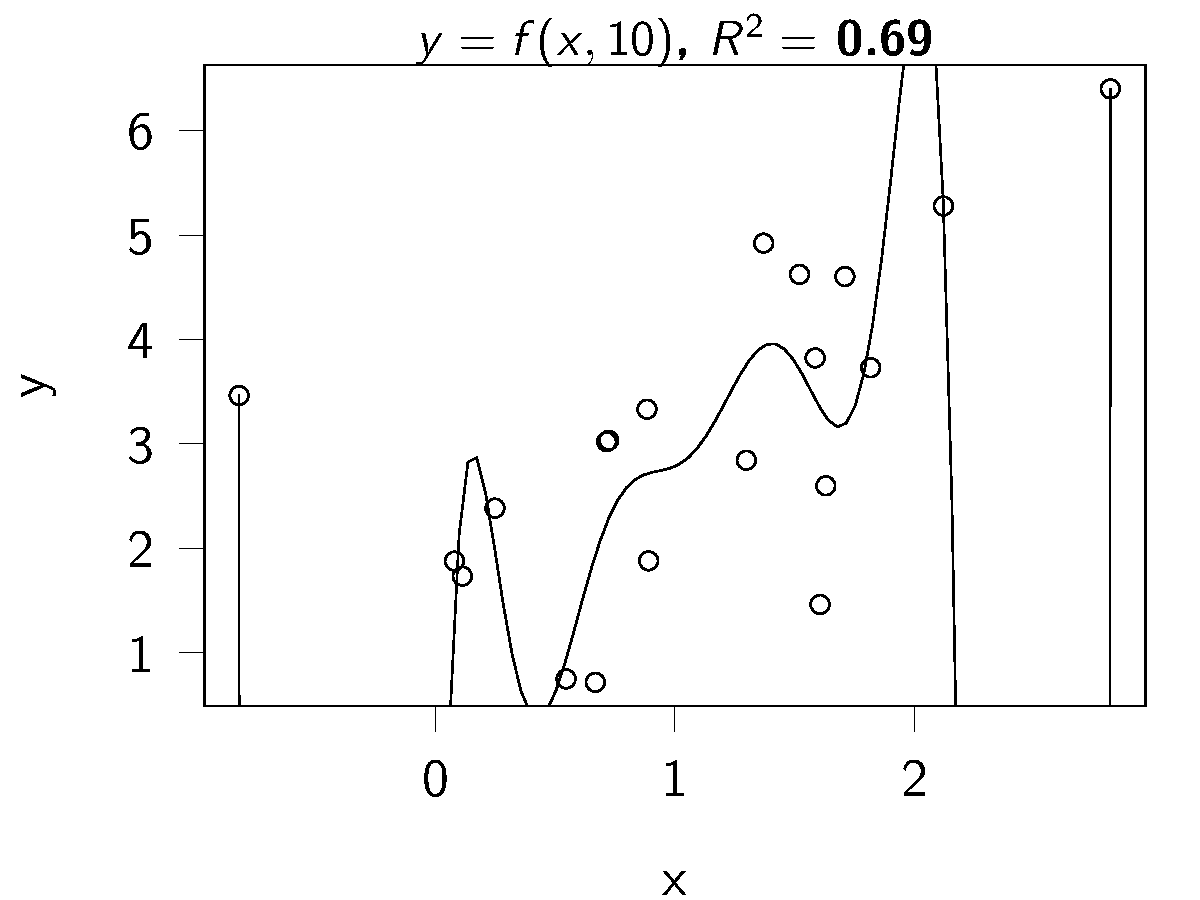
\includegraphics[width=0.8\textwidth,height=0.6\textwidth]{figure/model6b-1} 

\end{knitrout}
}

\only<2>{
\begin{knitrout}\small
\definecolor{shadecolor}{rgb}{0.843, 0.867, 0.922}\color{fgcolor}
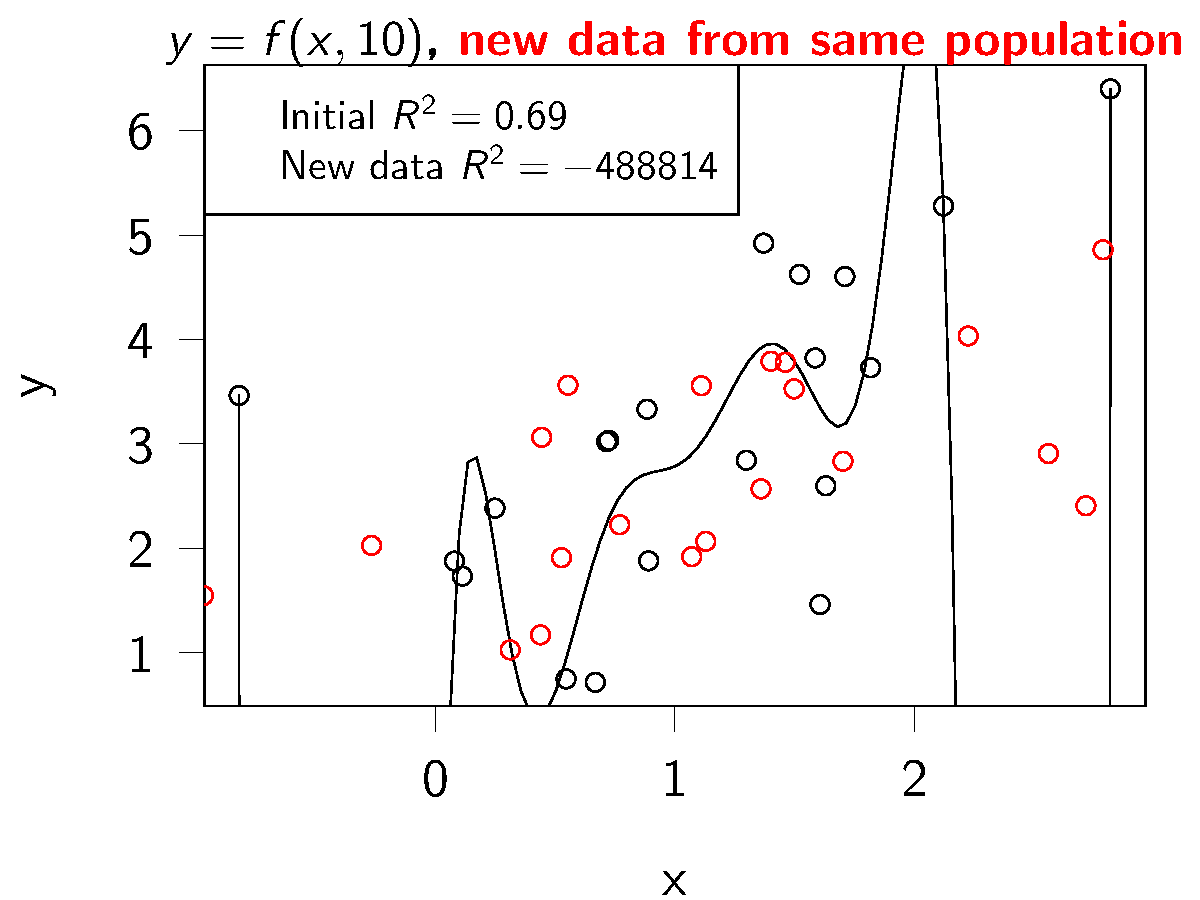
\includegraphics[width=0.8\textwidth,height=0.6\textwidth]{figure/model6c-1} 

\end{knitrout}
}
\end{frame}
%%%%%%%%%%

\begin{frame}{Overfitting: What is wrong? Part 2}

% latex table generated in R 3.6.0 by xtable 1.8-4 package
% Thu May 30 22:22:35 2019
\begin{table}[ht]
\centering
\begin{tabular}{rrrrr}
  \hline
 & Estimate & Std. Error & t value & p.value \\ 
  \hline
(Intercept) & -6.06 & 8.44 & -0.72 & 0.49 \\ 
  poly(x, 10, raw = TRUE)1 & 149.34 & 155.39 & 0.96 & 0.36 \\ 
  poly(x, 10, raw = TRUE)2 & -855.96 & 901.62 & -0.95 & 0.37 \\ 
  poly(x, 10, raw = TRUE)3 & 1984.17 & 2164.20 & 0.92 & 0.38 \\ 
  poly(x, 10, raw = TRUE)4 & -1647.96 & 1928.23 & -0.85 & 0.41 \\ 
  poly(x, 10, raw = TRUE)5 & -1070.35 & 1116.87 & -0.96 & 0.36 \\ 
  poly(x, 10, raw = TRUE)6 & 3444.36 & 3796.44 & 0.91 & 0.39 \\ 
  poly(x, 10, raw = TRUE)7 & -3113.36 & 3503.16 & -0.89 & 0.40 \\ 
  poly(x, 10, raw = TRUE)8 & 1416.27 & 1611.35 & 0.88 & 0.40 \\ 
  poly(x, 10, raw = TRUE)9 & -328.50 & 376.33 & -0.87 & 0.41 \\ 
  poly(x, 10, raw = TRUE)10 & 30.84 & 35.50 & 0.87 & 0.41 \\ 
   \hline
\end{tabular}
\end{table}


\end{frame}
%%%%%%%%%%

\begin{frame}{Overfitting: What is wrong}

\begin{alertblock}{Very good fit, but model USELESS}
\begin{itemize}
  \item Worse prediction than just taking the mean
  \item No biological interpretation
  \item Huge standar error, large p-values
\end{itemize}
\end{alertblock}

\end{frame}
%%%%%%%%%%%%%


\begin{frame}{``Less bias = More uncertainty"}
\centering
\begin{knitrout}\small
\definecolor{shadecolor}{rgb}{0.843, 0.867, 0.922}\color{fgcolor}
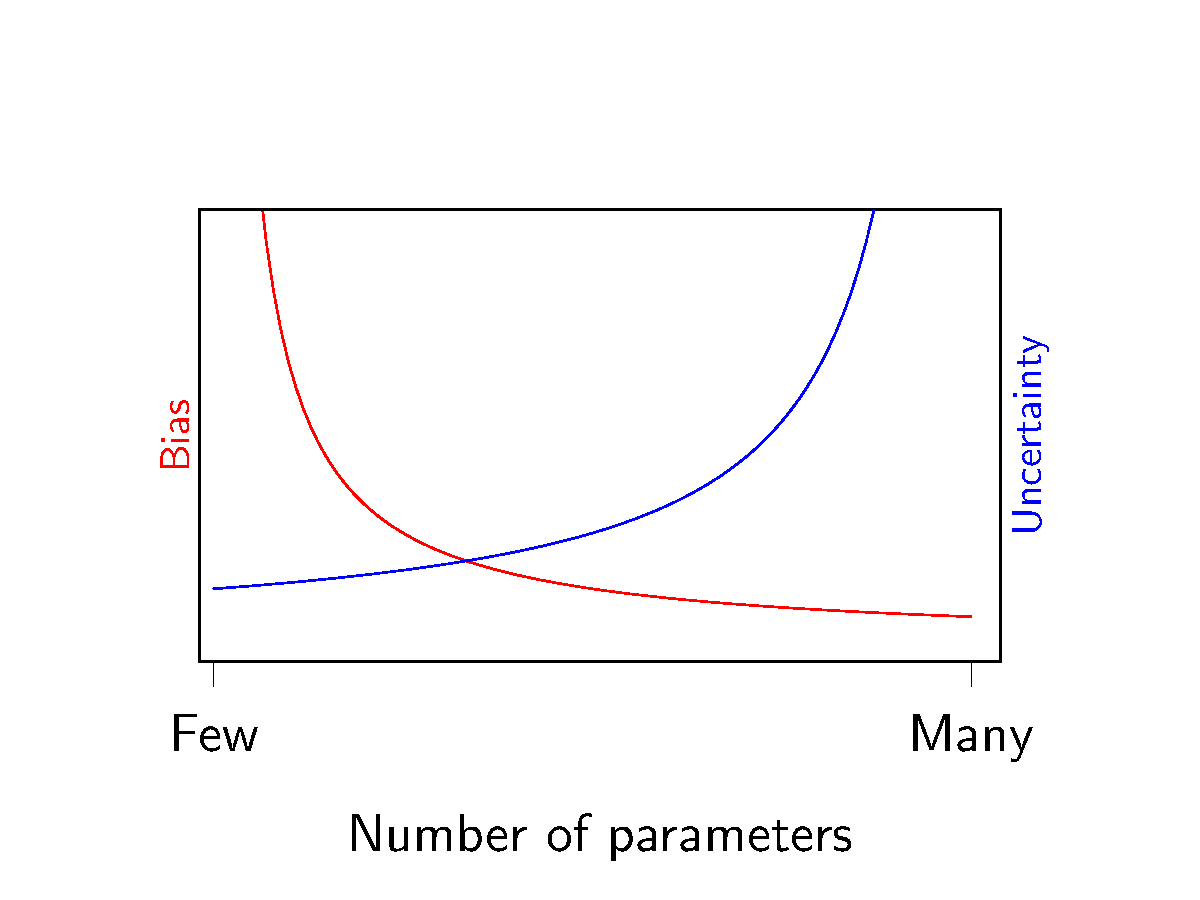
\includegraphics[width=0.8\textwidth,height=0.6\textwidth]{figure/unnamed-chunk-4-1} 

\end{knitrout}

\textbf{What is the best compromise?}

\end{frame}
%%%%%%%%%%

\begin{frame}{What is the best compromise?}

\begin{block}{Stepwise regression, one of multiple approaches:}
  Start from a simple model
  \begin{enumerate}
    \item Add covariates, once at the time, fit the models
    \item Keep the "most significant" covariate
    \item If no covariate is significant, stop
  \end{enumerate}
\end{block}



\end{frame}
%%%%%%%%%%%

\begin{frame}[fragile]{Try stepwise regression}


\begin{knitrout}\small
\definecolor{shadecolor}{rgb}{0.843, 0.867, 0.922}\color{fgcolor}\begin{kframe}
\begin{alltt}
\hlstd{datsub1} \hlkwb{<-} \hlkwd{read.csv}\hlstd{(}\hlstr{"datsub1.csv"}\hlstd{)}
\hlkwd{str}\hlstd{(datsub1)}
\end{alltt}
\end{kframe}
\end{knitrout}

\pause 

Stepwise selection part 1:\vspace{-0.1cm}
\begin{knitrout}\small
\definecolor{shadecolor}{rgb}{0.843, 0.867, 0.922}\color{fgcolor}\begin{kframe}
\begin{alltt}
\hlkwd{summary}\hlstd{(}\hlkwd{lm}\hlstd{(y} \hlopt{~} \hlstd{x1,} \hlkwc{data} \hlstd{= datsub1))}
\hlkwd{summary}\hlstd{(}\hlkwd{lm}\hlstd{(y} \hlopt{~} \hlstd{x2,} \hlkwc{data} \hlstd{= datsub1))}
\hlkwd{summary}\hlstd{(}\hlkwd{lm}\hlstd{(y} \hlopt{~} \hlstd{x3,} \hlkwc{data} \hlstd{= datsub1))}
\hlkwd{summary}\hlstd{(}\hlkwd{lm}\hlstd{(y} \hlopt{~} \hlstd{x4,} \hlkwc{data} \hlstd{= datsub1))}
\end{alltt}
\end{kframe}
\end{knitrout}

\pause

Stepwise selection part 2:\vspace{-0.1cm}
\begin{knitrout}\small
\definecolor{shadecolor}{rgb}{0.843, 0.867, 0.922}\color{fgcolor}\begin{kframe}
\begin{alltt}
\hlkwd{summary}\hlstd{(}\hlkwd{lm}\hlstd{(y} \hlopt{~} \hlstd{x2} \hlopt{+} \hlstd{x1,} \hlkwc{data} \hlstd{= datsub1))}
\hlkwd{summary}\hlstd{(}\hlkwd{lm}\hlstd{(y} \hlopt{~} \hlstd{x2} \hlopt{+} \hlstd{x3,} \hlkwc{data} \hlstd{= datsub1))}
\hlkwd{summary}\hlstd{(}\hlkwd{lm}\hlstd{(y} \hlopt{~} \hlstd{x2} \hlopt{+} \hlstd{x4,} \hlkwc{data} \hlstd{= datsub1))}
\end{alltt}
\end{kframe}
\end{knitrout}

\pause
Stepwise selection part 3: \vspace{-0.1cm}
\begin{knitrout}\small
\definecolor{shadecolor}{rgb}{0.843, 0.867, 0.922}\color{fgcolor}\begin{kframe}
\begin{alltt}
\hlkwd{summary}\hlstd{(}\hlkwd{lm}\hlstd{(y} \hlopt{~} \hlstd{x2} \hlopt{+} \hlstd{x4} \hlopt{+} \hlstd{x1,} \hlkwc{data} \hlstd{= datsub1))}
\hlkwd{summary}\hlstd{(}\hlkwd{lm}\hlstd{(y} \hlopt{~} \hlstd{x2} \hlopt{+} \hlstd{x4} \hlopt{+} \hlstd{x3,} \hlkwc{data} \hlstd{= datsub1))}
\end{alltt}
\end{kframe}
\end{knitrout}


\end{frame}
%%%%%%%%%%%%


\begin{frame}[fragile]{Try stepwise regression}
Based on this approach the best model is:
\begin{knitrout}\small
\definecolor{shadecolor}{rgb}{0.843, 0.867, 0.922}\color{fgcolor}\begin{kframe}
\begin{alltt}
\hlkwd{summary}\hlstd{(}\hlkwd{lm}\hlstd{(y} \hlopt{~} \hlstd{x2} \hlopt{+} \hlstd{x4,} \hlkwc{data} \hlstd{= datsub1))}
\end{alltt}
\end{kframe}
\end{knitrout}

Compare this to the full model:
\begin{knitrout}\small
\definecolor{shadecolor}{rgb}{0.843, 0.867, 0.922}\color{fgcolor}\begin{kframe}
\begin{alltt}
\hlkwd{summary}\hlstd{(}\hlkwd{lm}\hlstd{(y} \hlopt{~} \hlstd{x1} \hlopt{+} \hlstd{x2} \hlopt{+} \hlstd{x3} \hlopt{+} \hlstd{x4,} \hlkwc{data} \hlstd{= datsub1))}
\end{alltt}
\end{kframe}
\end{knitrout}

Which is best at predicting $y$ ? (you can use the function \texttt{predict() or look at the R-squared in summary()})

\end{frame}
%%%%%%%%%%%

\begin{frame}[fragile]{Try stepwise regression}
The full model explains more variation in $y$ in \texttt{datsub1}. But can we trust the full model for new data?
\pause

The dataset \texttt{datsub2} comes from the same population. Make predictions of $y$ in \texttt{datsub2} based on the best and the full models, and compare them to the true values of $y$ in \texttt{datsub2}. You could use the function \texttt{predict}, \texttt{plot}, and \texttt{cor}.

Start for the full model:
\begin{knitrout}\small
\definecolor{shadecolor}{rgb}{0.843, 0.867, 0.922}\color{fgcolor}\begin{kframe}
\begin{alltt}
\hlstd{datsub2} \hlkwb{<-} \hlkwd{read.csv}\hlstd{(}\hlstr{"datsub2.csv"}\hlstd{)}
\hlstd{predictedy} \hlkwb{<-} \hlkwd{predict}\hlstd{(}\hlkwd{lm}\hlstd{(y} \hlopt{~} \hlstd{x1} \hlopt{+} \hlstd{x2} \hlopt{+} \hlstd{x3} \hlopt{+} \hlstd{x4,} \hlkwc{data} \hlstd{= datsub1),}
                      \hlkwc{newdata} \hlstd{= datsub2)}
\end{alltt}
\end{kframe}
\end{knitrout}



\end{frame}
%%%%%%%%%%%%

\begin{frame}{Summary: Why model selection}

  \begin{exampleblock}{}
    \begin{itemize}
      \item Adding predictors increases fit to the response, in the current data
      \item But too many predictors:
        \begin{itemize}
          \item DECREASE fit in new data (from the same population)
          \item Hinder biological interpretation
          \item Increases esimtation uncertainty (larger SE and p-values)
        \end{itemize}
      \item Model selection aims to balance fit and generalisation 
    \end{itemize}
  \end{exampleblock}
\end{frame}
%%%%%%%%%%%

\section{Information criteria vs. stepwise selection}

\begin{frame}[fragile]{Model selection aims to balance fit and generalisation: How?}
  Stepwise regression is an option. But not very good.
  

  
Load \texttt{threepreddat.csv} and apply the previous stepwise regression method to model selection. What is the best model to predict the response?




  
\pause
Compare your best model to:
\begin{knitrout}\small
\definecolor{shadecolor}{rgb}{0.843, 0.867, 0.922}\color{fgcolor}\begin{kframe}
\begin{alltt}
\hlkwd{summary}\hlstd{(}\hlkwd{lm}\hlstd{(response} \hlopt{~} \hlstd{pred2} \hlopt{+} \hlstd{pred3,} \hlkwc{data} \hlstd{= threepreddat))}
\end{alltt}
\end{kframe}
\end{knitrout}
  
\end{frame}
%%%%%%%%%%%

\begin{frame}{Information criteria}

\begin{alertblock}{Do NOT use stepwise regression for model selection}
  \begin{itemize}
    \item Different version of stepwise regression often disagree
    \item Only nested models are compared 
    \item Sometimes the best models cannot be discovered stepwise
  \end{itemize}
\end{alertblock}

\pause

\begin{exampleblock}{Instead, use Information Criteria}
  \begin{itemize}[<+->]
    \item Akaike information criterion (AIC), invented in the 1970s, maximizes prediction
    \item Later BIC, DIC, TIC\dots maximizes different aspects of model performance
    \item AIC = 2$\times$Number of parameters - 2$\times \log(\text{model likelihood})$
    \item Smaller is better
    \item Only relative measure, no absolute meaning
  \end{itemize}
\end{exampleblock}

\end{frame}
%%%%%%%%%%%

\begin{frame}[fragile]{AIC in R}

Find the best AIC-model from \texttt{threepreddat}. For instance:

\begin{knitrout}\small
\definecolor{shadecolor}{rgb}{0.843, 0.867, 0.922}\color{fgcolor}\begin{kframe}
\begin{alltt}
\hlkwd{AIC}\hlstd{(}\hlkwd{lm}\hlstd{(response} \hlopt{~} \hlstd{pred1,} \hlkwc{data} \hlstd{= threepreddat))}
\end{alltt}
\begin{verbatim}
[1] 151.1339
\end{verbatim}
\end{kframe}
\end{knitrout}

\end{frame}
%%%%%%%%%%

\begin{frame}{AIC best practice:}
  
  False positives happen $\rightarrow$ \\ \hfill if you compare many models, ``spurious'' one can be best by pure chance
  
  \pause
  
  \begin{exampleblock}{Minimize the risks:}
  \begin{itemize}[<+->]
    \item Compare only models that make biological sense (e.g., avoid complex interactions)
    \item If you know enough, pre-select small set of models representing competing hypotheses
    \item \textbf{Confirmation:} AIC-model selection on half your dataset, then fit best model on the second half
    \item Acknowledge results are inconlusive is AIC-difference below 2 (or below 5)
  \end{itemize}
  \end{exampleblock}

\end{frame}
%%%%%%%%%%%

\begin{frame}{Practice: form groups of 2-3 people}

\begin{center}
  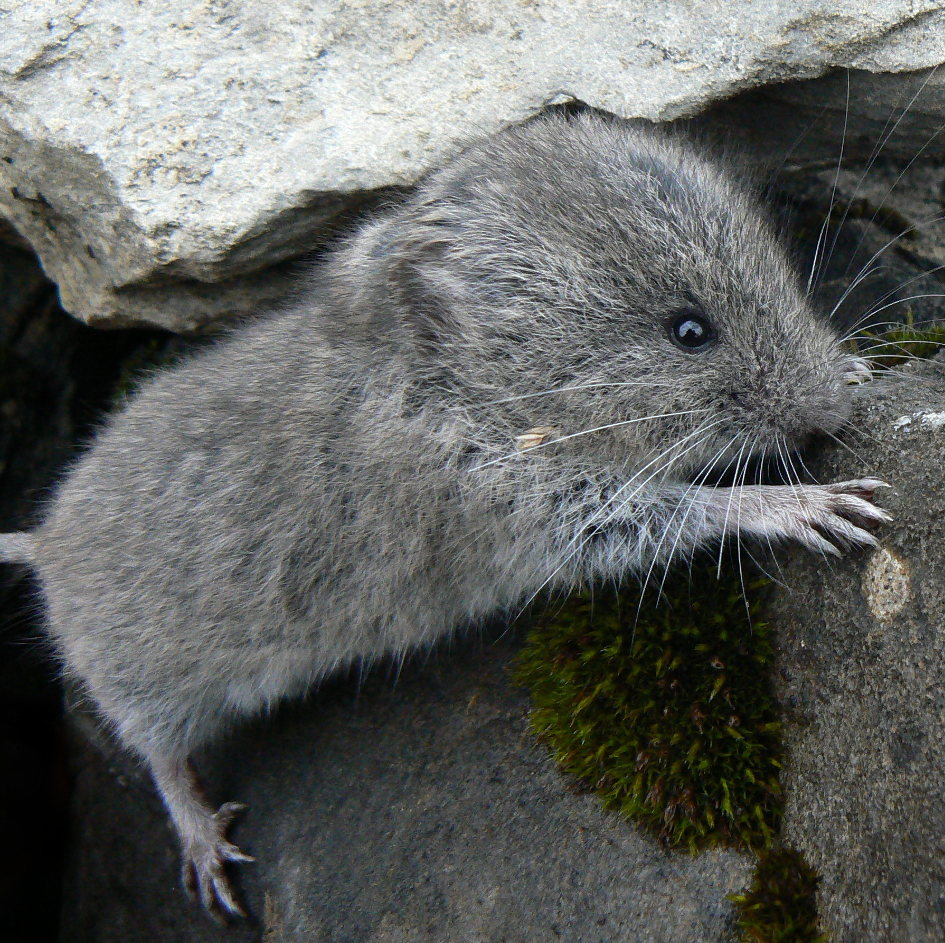
\includegraphics[width=0.4\textwidth]{Figures/vole}
\end{center}

Load \texttt{VoleWeight.csv}. We want to understand what factors explain variation in individual body weight. Think about what models could make sense. Use half the dataset for AIC comparison of those models. Check model performance on the second half.

\end{frame}
%%%%%%%%%%%

\begin{frame}{Summary: Information criteria vs. stepwise selection}
  \begin{exampleblock}{}
    \begin{itemize}[<+->]
      \item Stepwise 
        \begin{itemize}
          \item Different approches give inconsistent results
          \item compares only nested models
          \item \textbf{does NOT find the ``best'' model}
        \end{itemize}
      \item AIC 
        \begin{itemize}
          \item Compare all models, nested or not
          \item finds model best at predicting the response
          \item works better if competing models are pre-selected
        \end{itemize}
    \end{itemize}
  \end{exampleblock}
\end{frame}
%%%%%%%%%%%%%%%%%%%%%%%%%%%%%%%%%%%%%%%%%%%%%%%%%%%%%%%%%%%%%%%%%

\section{Model selection and causal inference}

\begin{frame}[fragile]{Competing hypotheses}



How does respiration rate scale with body mass in mammals? For a while researchers fought over two ideas, respiration could increase as a function of $mass^{2/3}$ or as a function of $mass^{3/4}$; while maybe the shape of the animals played a role. Let's find out!.

Load \texttt{metabo.csv} and compare models through AIC selection.

NB: you can fit exponents of a predictors using the function \texttt{I()}. For instance, for the exponent 0.5 of x:
\begin{knitrout}\small
\definecolor{shadecolor}{rgb}{0.843, 0.867, 0.922}\color{fgcolor}\begin{kframe}
\begin{alltt}
\hlkwd{lm}\hlstd{(y} \hlopt{~} \hlkwd{I}\hlstd{(x}\hlopt{^}\hlstd{(}\hlnum{1}\hlopt{/}\hlnum{2}\hlstd{)))}
\end{alltt}
\end{kframe}
\end{knitrout}

\end{frame}
%%%%%%%%%%%

\begin{frame}{Useful tools}
Package \texttt{MuMIn} useful for model selection

\begin{knitrout}\small
\definecolor{shadecolor}{rgb}{0.843, 0.867, 0.922}\color{fgcolor}\begin{kframe}
\begin{alltt}
\hlkwd{install.packages}\hlstd{(}\hlstr{"MuMIn"}\hlstd{)}
\hlkwd{library}\hlstd{(MuMIn)}
\end{alltt}
\end{kframe}
\end{knitrout}

\pause

\begin{exampleblock}{1. AICc}
  \begin{itemize}
    \item AIC is biased for small sample size
    \item AICc (``second-order AIC") when sample size / number of parameters is less than 40
    \item \texttt{MuMIn::AICc()}
  \end{itemize}
\end{exampleblock}

\pause

\begin{alertblock}{2. dredge}
  \begin{itemize}
    \item Automate model selection
    \item Convenient BUT many competing models, some may not make sense
    \item \texttt{MuMIn::dredge()}
  \end{itemize}
\end{alertblock}

\end{frame}
%%%%%%%%%%%

\begin{frame}{Try automated model selection}

Try to use \texttt{dredge()}, with selection based on \texttt{AICc}, to automate model selection on the vole data. 

For some reason you first need to run:
\begin{knitrout}\small
\definecolor{shadecolor}{rgb}{0.843, 0.867, 0.922}\color{fgcolor}\begin{kframe}
\begin{alltt}
\hlkwd{options}\hlstd{(}\hlkwc{na.action}\hlstd{=}\hlstr{"na.fail"}\hlstd{)}
\end{alltt}
\end{kframe}
\end{knitrout}


Do you find the same result?


\vfill

\textbf{If you get bored, go to next slide for a challenge!}
\end{frame}

\begin{frame}[fragile]{Challenge}
\small
In general, when a response variable is independent of the response there is a 5\% probability to find a p-value below 0.05 (that's a false positive).
Let's see for ourselves that it does not work if we do model selection first!

The code below creates one dataset with a response variable independent of the ``mainpredictor'' (the thing we want to test) and of control variables. We fit a full model, test many control variable combinations with \texttt{dredge()} and extract the p-value for ``mainpredictor''. Create a for-loop to look at the frequency of significant p-values!

\begin{knitrout}\small
\definecolor{shadecolor}{rgb}{0.843, 0.867, 0.922}\color{fgcolor}\begin{kframe}
\begin{alltt}
\hlstd{nobs} \hlkwb{<-} \hlnum{60}
\hlstd{mainpredictor} \hlkwb{<-} \hlkwd{rnorm}\hlstd{(nobs)}
\hlstd{control1} \hlkwb{<-} \hlkwd{rnorm}\hlstd{(nobs) ; control2} \hlkwb{<-} \hlkwd{rnorm}\hlstd{(nobs)}
\hlstd{control3} \hlkwb{<-} \hlkwd{rnorm}\hlstd{(nobs) ; control4} \hlkwb{<-} \hlkwd{rnorm}\hlstd{(nobs)}
\hlstd{control5} \hlkwb{<-} \hlkwd{rnorm}\hlstd{(nobs) ; response} \hlkwb{<-} \hlkwd{rnorm}\hlstd{(nobs)}

\hlstd{mfull} \hlkwb{<-} \hlkwd{lm}\hlstd{(response} \hlopt{~} \hlstd{mainpredictor} \hlopt{+}
              \hlstd{control1}\hlopt{*}\hlstd{control2}\hlopt{*}\hlstd{control3} \hlopt{+} \hlstd{control4}\hlopt{*}\hlstd{control5)}

\hlstd{modall} \hlkwb{<-} \hlkwd{dredge}\hlstd{(mfull,} \hlkwc{fixed} \hlstd{=} \hlstr{"mainpredictor"}\hlstd{)}
\hlkwd{summary}\hlstd{(}\hlkwd{get.models}\hlstd{(modall,} \hlnum{1}\hlstd{)[[}\hlnum{1}\hlstd{]])}\hlopt{$}\hlstd{coefficients[}\hlnum{2}\hlstd{,}\hlnum{4}\hlstd{]}\hlcom{#the pvalue}
\end{alltt}
\end{kframe}
\end{knitrout}


\end{frame}
%%%%%%%%%%%

\begin{frame}{``There is madness in our methods"}
\begin{figure}
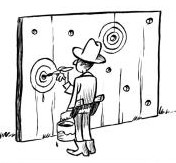
\includegraphics[width=0.5\textwidth]{Figures/dirk-jan-hoek}
\caption{Null-hypothesis testing after model selection \copyright Dirk Jan-Hoek}
\end{figure}

\url{https://methodsblog.com/2015/11/26/madness-in-our-methods/}
\end{frame}
%%%%%%%%%%%


\begin{frame}{Summary: Model selection and inference}

  \begin{exampleblock}{}
    \begin{itemize}
      \item AIC/AICc best for exploratory / predictive models
      \item AIC/AICc alone can be used for causal inference if models are all meaningful competing biological hypotheses
      \item After AIC/AICc selection p-values are wrong
      \item Correct p-values and standard errors MUST be computed on new data (Confirmatory model)
    \end{itemize}
  \end{exampleblock}
  
\end{frame}

%%%%%%%%%%%%%%%%%%%%%%%%%%%%%%%%%%%%%%%%%%%%%%%%%%%%%%%%%%%%%%%%%

\begin{frame}{Want more practice? }
\begin{block}{Use AIC/AICc to:}
  \begin{itemize}
    \item Tell what drives the increase in number of babies in \texttt{babies.csv}
    \item What drives bird abundance (ABUND) in \texttt{loyn.csv}
    \item \textbf{Challenge:} How do differences in AIC between nested models scale with p-values for the extra predictor?
  \end{itemize}
\end{block}

\end{frame}

\begin{frame}{Want to know more?}

\begin{exampleblock}{Very good, but very pro:}
  \begin{itemize}
    \item Burnham and Anderson, 2002, Model Selection and Multimodel Inference: A Practical Information-theoretic Approach
  \end{itemize}
\end{exampleblock}

\begin{alertblock}{AIC is not always the best choice:}
\begin{itemize}
  \item \textbf{``Your goal matters in the choice between AIC, BIC, p-values...:"} Aho \& al. A graphical framework for model selection criteria and significance tests: Refutation, confirmation and ecology. Methods in Ecology and Evolution. 2017;8:47–56.
  \item \textbf{``Careful when combining estimates from different models"}: Cade. Model averaging and muddled multimodel inferences. Ecology. 2015;96(9):2370–82.
\end{itemize}
\end{alertblock}

\end{frame}
%%%%%%%%%%

\begin{frame}{Before you leave:}
  \begin{enumerate}
    \item Write one thing you liked and one you disliked on a sticky note
    \item Be sure you signed the presence sheet, especially if you want credit for the HDR career development framework
    \item Leave your email address if you want to join the Slack channel 
    \item Past workshops at \url{https://timotheenivalis.github.io/RSB-R-Stats-Biology/} 
  \end{enumerate}

\vfill
\hfill Thank you!!

\end{frame}

\end{document}
